\documentclass{article}
\usepackage[svgnames]{xcolor}
\usepackage[british]{babel}
\usepackage[protrusion,expansion,tracking,kerning,babel,final]{microtype}
\usepackage[margin=1in]{geometry}
\usepackage[pdfversion=1.7]{hyperref}
\usepackage[shortlabels]{enumitem}
\usepackage{graphicx}
\usepackage{mathtools}
\usepackage{cleveref}
\usepackage{booktabs}
\usepackage{nicematrix}
\usepackage{derivative}
\usepackage{etoolbox}
\usepackage{siunitx}
\usepackage{bm}
\usepackage[T1]{fontenc}
\usepackage{multirow}

% Functions
\providecommand\given{} % just to make sure it exists
\DeclarePairedDelimiterXPP{\E}[1]{\operatorname{\text{E}}}[]{}{%
    \renewcommand\given{\nonscript\:\delimsize\vert\nonscript\:\mathopen{}}%
    \ifblank{#1}{\:\cdot\:}%
    #1}%
\DeclarePairedDelimiterXPP{\V}[1]{\operatorname{\Field{V}}}(){}{%
    \renewcommand\given{\nonscript\:\delimsize\vert\nonscript\:\mathopen{}}%
    \ifblank{#1}{\:\cdot\:}%
    #1}%
\DeclarePairedDelimiterXPP{\Var}[1]{\operatorname{\text{Var}}}(){}{%
    \renewcommand\given{\nonscript\:\delimsize\vert\nonscript\:\mathopen{}}%
    \ifblank{#1}{\:\cdot\:}%
    #1}%
\DeclarePairedDelimiterXPP{\Cov}[1]{\operatorname{\text{Cov}}}(){}{%
    \renewcommand\given{\nonscript\:\delimsize\vert\nonscript\:\mathopen{}}%
    \ifblank{#1}{\:\cdot\:}%
    #1}%
\DeclarePairedDelimiterXPP\Prob[1]{\operatorname{\Field{P}}}(){}{%
    \renewcommand\given{\nonscript\:\delimsize\vert\nonscript\:\mathopen{}}%
    \ifblank{#1}{\:\cdot\:}%
    #1}%
\DeclarePairedDelimiterXPP\Ind[1]{\operatorname{\Field{I}}}\{\}{}{%
    \renewcommand\given{\nonscript\:\delimsize\vert\nonscript\:\mathopen{}}%
    \ifblank{#1}{\:\cdot\:}%
    #1}%
\DeclarePairedDelimiterXPP{\se}[1]{\operatorname{\text{se}}}(){}{%
    \ifblank{#1}{\:\cdot\:}%
    #1}%
\DeclarePairedDelimiterXPP{\estse}[1]{\widehat{\operatorname{\text{se}}}}(){}{%
    \ifblank{#1}{\:\cdot\:}%
    #1}%
\DeclarePairedDelimiterXPP{\estV}[1]{\widehat{\operatorname{\Field{V}}}}(){}{
    \renewcommand\given{\nonscript\:\delimsize\vert\nonscript\:\mathopen{}}%
    \ifblank{#1}{\:\cdot\:}%
    #1}%
\DeclarePairedDelimiterXPP{\estVar}[1]{\widehat{\operatorname{\text{Var}}}}(){}{
    \renewcommand\given{\nonscript\:\delimsize\vert\nonscript\:\mathopen{}}%
    \ifblank{#1}{\:\cdot\:}%
    #1}%
\let\exp\relax%
\let\log\relax%
\let\ln\relax%
\DeclarePairedDelimiterXPP{\exp}[1]{\operatorname{\text{exp}}}\{\}{}{#1}%
\DeclarePairedDelimiterXPP{\log}[1]{\operatorname{\text{log}}}(){}{#1}%
\DeclarePairedDelimiterXPP{\ln}[1]{\operatorname{\text{ln}}}(){}{#1}%
\DeclarePairedDelimiterXPP{\diag}[1]{\operatorname{\text{diag}}}(){}{#1}%
\DeclarePairedDelimiterXPP{\sign}[1]{\operatorname{\text{sign}}}(){}{#1}%

\DeclarePairedDelimiterXPP{\expit}[1]{\operatorname{\text{expit}}}(){}{#1}%
\DeclarePairedDelimiterXPP{\logit}[1]{\operatorname{\text{logit}}}(){}{#1}%
\newcommand{\HN}{\text{H}_0}%
\newcommand{\HA}{\text{H}_{\text{A}}}%

% Distributions
\DeclarePairedDelimiterXPP{\N}[1]{\mathcal{N}}(){}{#1}%
\DeclarePairedDelimiterXPP{\Poisson}[1]{\text{Poisson}}(){}{#1}%
\DeclarePairedDelimiterXPP{\Bin}[1]{\text{Bin}}(){}{#1}%
\DeclarePairedDelimiterXPP{\Binomial}[1]{\text{Binomial}}(){}{#1}%
\DeclarePairedDelimiterXPP{\Bernoulli}[1]{\text{Bernoulli}}(){}{#1}%
\DeclarePairedDelimiterXPP{\MVN}[1]{\text{MVN}}(){}{#1}%

\newcommand{\iid}{\overset{\text{iid}}{\sim}}%
\newcommand{\ind}{\overset{\text{ind}}{\sim}}%
\newcommand{\OR}{\text{OR}}%
\newcommand{\RR}{\text{RR}}%

\DeclarePairedDelimiter\abs{\lvert}{\rvert}
% can be useful to refer to this outside \Set
\newcommand\SetSymbol[1][]{%
    \nonscript\:#1\vert{}
    \allowbreak\nonscript\:
    \mathopen{}}
\DeclarePairedDelimiterX\Set[1]\{\}{%
    \renewcommand\given{:}
    #1
}
\DeclareMathOperator*{\argmax}{arg\,max}
\DeclareMathOperator*{\argmin}{arg\,min}
\DeclareMathOperator*{\arginf}{arg\,inf}
\DeclareMathOperator*{\argsup}{arg\,sup}

% Table of Contents
\hypersetup{colorlinks,linkcolor=[rgb]{0,0.5,1}}%

\title{%
    {\LARGE Generalized Linear Models}\\%
    {\large STAT 431/STAT 831}\\%
    {\normalsize Spring 2022 (idk)}%
}%
\author{%
    \LaTeX{}er: \emph{Cameron Roopnarine}\\%
    Instructor: \emph{Leilei Zeng}%
}%
\date{\today}%

\providecommand{\RandomVector}[1]{\bm{#1}}% general vectors in bold italic
\providecommand{\Vector}[1]{\bm{#1}}% general vectors in bold italic
\providecommand{\Matrix}[1]{\bm{#1}}
\providecommand{\MatrixCal}[1]{\bm{\mathcal{#1}}}
\providecommand{\Field}[1]{\bm{#1}}

\usepackage{stackengine}
\usepackage[british]{isodate}
\newcommand{\makeheading}[2]%
{%
\begin{center}%
    \makebox[\linewidth]{\raisebox{-.5ex}[0cm][0cm]{\stackanchor{\textcolor{Gray}{\textsc{#1}}}{\scriptsize\itshape\printyearoff #2}\;}\color{Crimson!50}\hrulefill}%
\end{center}%
}%

\usepackage[breakable]{tcolorbox}
\tcbset{
    regular/.style={
        boxrule=0pt,
        breakable,
        sharp corners,
    }
}

\newtcolorbox{Example}[1]{regular,colframe=Green!20!white,colback=Green!10!white,coltitle=Green,title={#1}}%
\newtcolorbox{Regular}[1]{regular,colframe=Navy!15!white,colback=Navy!5!white,coltitle=Navy,title={#1}}%
\newtcolorbox{Result}[1]{regular,colframe=Red!15!white,colback=Red!5!white,coltitle=Red,title={#1}}%

\hypersetup{colorlinks=true,%
linkcolor=[rgb]{0,0.5,1},%
pdftitle={Introduction to Biostatistics (STAT 337)},%
pdfauthor={Cameron Roopnarine, Cecilia Cotton},%
pdfsubject={Statistics},%
pdfkeywords={University of Waterloo, Fall 2021 (1219)}}%

\title{%
\LARGE Introduction to Biostatistics\\%
\large STAT 337\\%
\normalsize Fall 2021 (1219)\thanks{Online Course}}%
\author{Cameron Roopnarine\thanks{\LaTeX{}er}\and Cecilia Cotton\thanks{Instructor}}%
\date{\today}%

\begin{document}
\maketitle
\newpage
\tableofcontents
\newpage
\chapter{Integration}
\setcounter{section}{1}
\section{Riemann Sums and the Definite Integral}
To begin with, our goal is to develop methods for determining the area under a curve.

We know we can approximate the area using rectangles (or other geometric shapes), but
we want the \emph{exact} area. For this, we will need \emph{Riemann sums}.

\begin{Definition}{Partition}{partition}
    A \textbf{partition}, $P$, for the interval $ \interval{a}{b} $ is a finite
    sequence of increasing numbers of the form
    \[ a=t_0<t_1<t_2\cdots<t_{n-1}<t_n=b \]
    This partition subdivides the interval $ \interval{a}{b} $ into $ n $ subintervals:
    \[ \interval{t_0}{t_1},\ldots,\interval{t_{n-1}}{t_n} \]
\end{Definition}

\begin{Remark}{}{}
    These subintervals may \emph{not} all have the same length.
\end{Remark}

\begin{Definition}{Length}{length}
    Denote the \textbf{length} of the $ i^{\text{th}} $ subinterval,
    $ \interval{t_{i-1}}{t_i} $, by $ \Delta t_i $; that is, $ \Delta t_i=t_i-t_{i-1} $.
\end{Definition}

\begin{Definition}{Norm}{norm}
    The \textbf{norm} of a partition is the length of the widest subinterval:
    \[ \norm{P}=\max(\Delta t_1,\dots,\Delta t_{n}) \]
\end{Definition}

\begin{Definition}{Riemann sum}{riemann_Sum}
    Given a bounded function $ f $ on $ \interval{a}{b} $,
    a partition $ P $ of $ \interval{a}{b} $, and a set
    $ \set{c_1,\dots,c_n} $, where $ c_i\in\interval{t_{i-1}}{t_i} $, then a
    \textbf{Riemann sum} for $ f $ with respect to $ P $ is
    \[ S=\sum\limits_{i=1}^{n} f(c_i)\Delta t_i \]
\end{Definition}

Again, we want the \emph{exact} area, and for that we will need to use infinitely
many points!

But we do need to make sure that the norm of our partitions is getting smaller,
and that the area we get doesn't depend on the choice of Riemann sum.

\begin{Definition}{Integrable, Integral of $ f $}{integrable}
    We say that $ f $ is \textbf{integrable} on $ \interval{a}{b} $ if there exists a unique number
    $ I\in\mathbb{R} $ such that if whenever $ \set{P_n} $ is a sequence of partitions with
    $ \lim\limits_{{n} \to {\infty}}\norm{P_n}=0 $ and $ \set{S_n} $ is any sequence of
    Riemann sums associated to the $ P_n $'s, we have $ \lim\limits_{{n} \to {\infty}} S_n=I $.

    In this case, we call $ I $ the \textbf{integral of $ f $} over $ \interval{a}{b} $
    and denote it by
    \[ \int_{a}^{b} f(x)\, dx \]
    where $ a,b $ are the bounds of integration, $ f(x) $ is the integrand, $ x $ is the
    variable of integration. The complete object is called a definite integral.

    It represents the exact (signed) area under $ f $.
\end{Definition}

\begin{Remark}{}{}
    The variable of integration is a \emph{dummy variable} since we can change it into
    whatever we want and it won't change the value of the integral; that is,
    \[
        \int_{a}^{b} f(x)\,dx =
        \int_{a}^{b} f(t) \,d{t}=
        \int_{a}^{b} f(\cdot)\, d{\cdot}
    \]
\end{Remark}

This looks \emph{horrible} to compute in practice (and it is). The good news is if
$ f $ is continuous, it's not so bad! (still bad though)

\begin{Theorem}{Integrability Theorem for Continuous Functions}{integrability_thm}
    Let $ f $ be continuous on $ \interval{a}{b} $.
    Then $ f $ is integrable on $ \interval{a}{b} $.
\end{Theorem}

\begin{Proof}{\ref{thm:integrability_thm}}{}
    Beyond the scope of this course.
\end{Proof}

This is fantastic! This means that we can \emph{choose} any collection of Riemann sums
we want when computing the integral of a continuous function!

Let's examine a ``nice'' choice: one where the partition is regular and where we just
pick the $ c_i $'s to be the right-hand endpoints!

\begin{Definition}{Regular $n$-partition}{regular_partition}
    For the interval $ \interval{a}{b} $, the \textbf{regular $ n $-partition}
    where all $ n $ subintervals
    have the same length; that is,
    \[ \Delta t=\frac{b-a}{n} \quad\text{and}\quad  t_i=t_0+i\Delta t \]
\end{Definition}

\begin{Definition}{Regular right-hand Riemann sum}{right_hand_reimann}
    Using this, we define the \textbf{regular right-hand Riemann sum} by taking $ c_i=t_i $ for
    all $ i $:
    \[ S_n=\sum\limits_{i=1}^{n} f(t_i)\Delta t=\sum\limits_{i=1}^{n} f(t_i)\left(\frac{b-a}{n}\right) \]
\end{Definition}

\begin{Remark}{}{}
    We can also define the regular left-hand Riemann sum.
\end{Remark}

Now, we can write a nicer formula for integrating continuous functions!

If $ f $ is continuous, then
\[ \boxed{\int_{a}^{b} f(x)\, d{x} =
        \lim\limits_{{n} \to {\infty}} \sum\limits_{i=1}^{n} f(t_i)\left(\frac{b-a}{n}\right)} \]

\begin{Example}{}{}
    Evaluate
    $ \displaystyle\int_{0}^{4} x+x^3\, d{x} $.

    \textbf{Solution.}
    Since $ f(x)=x+x^3 $ is continuous, we can use the above formula.

    In our case: $ \dfrac{b-a}{n} = \dfrac{4}{n} $, and $ t_i = 0+\dfrac{4i}{n} = \dfrac{4i}{n} $.

    So, $ f(t_i) = \dfrac{4i}{n} + \dfrac{64i^3}{n^3} $.
    Then, we get:
    \begin{align}
        \int_{0}^{4} x+x^3\, d{x}
         & = \lim\limits_{{n} \to {\infty}} \sum\limits_{i=1}^{n}
        \left( \frac{4i}{n} +\frac{64i^3}{n^3} \right)\left( \frac{4}{n} \right)                  \\
         & = \lim\limits_{{n} \to {\infty}} \frac{16}{n^2} \sum\limits_{i=1}^{n} i +
        \frac{256}{n^4} \sum\limits_{i=1}^{n} i^3 \label{1.2_reimann}                             \\
         & = \lim\limits_{{n} \to {\infty}} \frac{16}{n^2} \left[ \frac{n(n+1)}{2} \right] +
        \frac{256}{n^4} \left[ \frac{n^2(n+1)^2}{4} \right] \label{1.3_reimann}                   \\
         & = \lim\limits_{{n} \to {\infty}} \frac{8n+8}{n} +64 \left(\frac{n^2+2n+1}{n^2} \right) \\
         & = 8+64                                                                                 \\
         & =72
    \end{align}
    where from~\ref{1.2_reimann} to~\ref{1.3_reimann} we used both of the following:
    \[ \sum\limits_{i=1}^{n} i=\frac{n(n+1)}{2} \text{ and }
        \sum\limits_{i=1}^{n} i^3=\frac{n^2(n+1)^2}{4} \]
\end{Example}

\begin{Remark}{}{}
    The theorem also holds for functions that are bounded and have finitely many
    discontinuities.
\end{Remark}

\section{Properties of the Definite Integral}

Since a definite integral is the limit of a sequence, many limit laws also hold!

\begin{Theorem}{Properties of Integrals}{properties_of_integrals}
    Assume that $ f $ and $ g $ are integrable on the interval $ \interval{a}{b} $. Then:
    \begin{enumerate}[label=(\arabic*)]
        \item\label{property_integral_1} For any $ c\in\mathbb{R} $,
              $ \displaystyle\int_{a}^{b} cf(x)\, d{x} = c \int_{a}^{b} f(x)\, d{x} $.
        \item\label{property_integral_2}
              $ \displaystyle \int_{a}^{b} (f+g)(x)\, d{x} = \int_{a}^{b} f(x)\, d{x} +
                  \int_{a}^{b} g(x)\, d{x} $.
        \item\label{property_integral_3} If $ m\le f(x)\le M $ for all $ x\in\interval{a}{b} $,
              then
              $ \displaystyle m(b-a)\le \int_{a}^{b} f(x)\, d{x} \le M(b-a) $.
        \item\label{property_integral_4} If $ 0\le f(x) $ for all $ x\in\interval{a}{b} $, then
              $ \displaystyle 0\le \int_{a}^{b} f(x)\, d{x} $.
        \item\label{property_integral_5} If $ f(x)\le g(x) $ for all $ x\in\interval{a}{b} $, then
              $ \displaystyle \int_{a}^{b} f(x)\, d{x} \le \int_{a}^{b} g(x)\, d{x} $.
        \item\label{property_integral_6} The function
              $ \abs{f} $ is integrable on $ \interval{a}{b} $ and
              $ \displaystyle \abs[\bigg]{\int_{a}^{b} f(x)\, d{x}}
                  \le \int_{a}^{b} \abs{f(x)}\, d{x} $.
    \end{enumerate}
\end{Theorem}

\begin{Proof}{\ref{thm:properties_of_integrals}}{}
    \begin{itemize}
        \item~\ref{property_integral_1} and~\ref{property_integral_2} follow from limit laws
              for sequences.
        \item~\ref{property_integral_3} implies~\ref{property_integral_4}.
        \item~\ref{property_integral_1},~\ref{property_integral_2},
              and~\ref{property_integral_4} imply~\ref{property_integral_5}.
        \item~\ref{property_integral_6} follows from the triangle inequality.
    \end{itemize}

    We will now prove~\ref{property_integral_3}.

    Suppose $ m\le f(x)\le M $ and partition the interval
    $ a=t_0<\cdots<t_n=b $.

    Note that
    $ \displaystyle\sum\limits_{i=1}^{n} \Delta t=\frac{b-a}{n}(n)=b-a $
    Then, since $ m\le f(x)\le M $, we get
    \[ m(b-a)=\sum\limits_{i=1}^{n} m\Delta t\le \sum\limits_{i=1}^{n} f(t_i)\Delta t
        \le \sum\limits_{i=1}^{n} M\Delta t=M(b-a) \]
    So, taking limits gives
    \[ m(b-a)\le \int_{a}^{b} f(x)\,d{x} \le M(b-a) \]
\end{Proof}

\begin{Definition}{More properties}{more_properties}
    \begin{enumerate}[label=(\Roman*)]
        \item If $ f(a) $ is defined, then
              $ \displaystyle\int_{a}^{a} f(x)\, d{x} =0 $
        \item If $ f $ is integrable on $ \interval{a}{b} $, then
              $ \displaystyle\int_{a}^{b} f(x)\, d{x}=-\int_{b}^{a} f(x)\, d{x} $
    \end{enumerate}
\end{Definition}

\begin{Theorem}{}{extra_integ_property}
    If $ f $ is integrable on an interval $ I $ containing $ a,b $, and $ c $, then
    \[ \int_{a}^{b} f(x)\, d{x}=\int_{a}^{c} f(x)\, d{x}+\int_{c}^{b} f(x)\, d{x} \]
\end{Theorem}

\begin{Proof}{\ref{thm:extra_integ_property}}{}
    Beyond the scope of this course.
\end{Proof}

\begin{Remark}{}{}
    $ c $ does \emph{not} need to be between $ a $ and $ b $!
\end{Remark}

\subsection*{Geometric Interpretation of the Integral}
So far, we have only examined positive functions, but we should note that $ \int_{a}^{b} f(x)\,dx $
returns the \emph{signed} area between $ f $ and the $ x $-axis. That is, if $ f(x)\le 0 $, then
$ \int_{a}^{b} f(x)\,dx\le 0 $ too.

So, in general, $ \int_{a}^{b} f(x)\,dx $ is the area under $ f $ that
lies above the $ x $-axis \emph{minus} the area above the graph of
$ f $ that lies below the $ x $-axis.

\begin{Example}{}{}
    \[ \int_{-1}^{1}x\,dx=R_2-R_1 \]
    but $ R_2=R_2 $, so
    \[ \int_{-1}^{1}x\,dx=0 \]
    \begin{figure}[H]
        \centering
        \tikzset{every picture/.style={line width=0.75pt}} %set default line width to 0.75pt        

        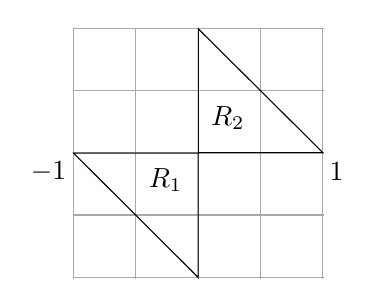
\begin{tikzpicture}[x=0.75pt,y=0.75pt,yscale=-1,xscale=1]
            %Shape: Grid [id:dp8044758903954956] 
            \draw  [draw opacity=0] (252.83,80.33) -- (373.67,80.33) -- (373.67,201.33) -- (252.83,201.33) -- cycle ; \draw  [color={rgb, 255:red, 168; green, 168; blue, 168 }  ,draw opacity=1 ] (252.83,80.33) -- (252.83,201.33)(282.83,80.33) -- (282.83,201.33)(312.83,80.33) -- (312.83,201.33)(342.83,80.33) -- (342.83,201.33)(372.83,80.33) -- (372.83,201.33) ; \draw  [color={rgb, 255:red, 168; green, 168; blue, 168 }  ,draw opacity=1 ] (252.83,80.33) -- (373.67,80.33)(252.83,110.33) -- (373.67,110.33)(252.83,140.33) -- (373.67,140.33)(252.83,170.33) -- (373.67,170.33)(252.83,200.33) -- (373.67,200.33) ; \draw  [color={rgb, 255:red, 168; green, 168; blue, 168 }  ,draw opacity=1 ]  ;
            %Shape: Right Triangle [id:dp6090851976145147] 
            \draw   (313,80.67) -- (373,140.33) -- (313,140.33) -- cycle ;
            %Shape: Right Triangle [id:dp2511359111159521] 
            \draw   (312.83,200.33) -- (252.83,140.5) -- (312.83,140.5) -- cycle ;

            % Text Node
            \draw (375,143.73) node [anchor=north west][inner sep=0.75pt]    {$1$};
            % Text Node
            \draw (231,143.4) node [anchor=north west][inner sep=0.75pt]    {$-1$};
            % Text Node
            \draw (287.83,146.73) node [anchor=north west][inner sep=0.75pt]    {$R_{1}$};
            % Text Node
            \draw (317.83,116.73) node [anchor=north west][inner sep=0.75pt]    {$R_{2}$};
        \end{tikzpicture}
    \end{figure}
\end{Example}

\begin{Remark}{}{}
    If we are lucky, we can use geometric formulas to evaluate integrals
    (see pg 26--28 in the notes). However, we are almost never this lucky\textellipsis{}
\end{Remark}

\section{Average Value of a Function}

\begin{Definition}{Average value}{avg_value}
    If $ f $ is continuous on $ \interval{a}{b} $, the \textbf{average value} of $ f $
    on $ \interval{a}{b} $ is defined as
    $ \displaystyle \frac{1}{b-a} \int_{a}^{b} f(x)\,dx $.
\end{Definition}

\subsection*{Geometric Interpretation}
\begin{Proof}{\ref{thm:avt}}{}
    If $ f $ is continuous on $ \interval{a}{b} $, EVT says there exists $ m,M\in\mathbb{R} $ such that
    $ \displaystyle m\le f(x) \le M $
    for $ x\in\interval{a}{b} $, and $ f(c_1)=m $, $ f(c_2)=M $ for some $ c_1,c_2\in\interval{a}{b} $.

    Also, we know
    \begin{align*}
        m(b-a)\le \int_{a}^{b} f(x)\, d{x} \le M(b-a)
         & \implies m\le \frac{1}{b-a} \int_{a}^{b} f(x)\, d{x} \le M       \\
         & \iff f(c_1)\le \frac{1}{b-a} \int_{a}^{b} f(x)\, d{x} \le f(c_2) \\
    \end{align*}
    IVT says there exists $ c $ between $ c_1 $ and $ c_2 $, so that
    \[ f(c)=\frac{1}{b-a} \int_{a}^{b} f(x)\, d{x} \]
\end{Proof}

\begin{Theorem}{Average Value Theorem (AVT)}{avt}
    Assume $ f $ is continuous on $ \interval{a}{b} $.
    There exists $ c\in\interval{a}{b} $ such that
    $ \displaystyle f(c)=\frac{1}{b-a} \int_{a}^{b} f(x) d{x} $.
\end{Theorem}

\begin{Remark}{}{}
    Note that this theorem holds even if $ b<a $ since
    \begin{align*}
        f(c) & =\frac{1}{a-b} \int_{b}^{a}\, f(x)dx                  \\
             & =\frac{1}{a-b}\biggl(-\int_{a}^{b} f(x)\, d{x}\biggr) \\
             & =\frac{1}{b-a} \int_{a}^{b} f(x)\, d{x}
    \end{align*}
\end{Remark}

The big problem we face now is that evaluating $ \int_{a}^{b} f(x)\, d{x} $ is
monstrously difficult for all but the simplest of functions.

IF ONLY THERE WAS A BETTER WAY\@!

(spoilers: there's a better way! It's the Fundamental Theorem of Calculus!)



\end{document}
